\documentclass[../diploma.tex]{subfiles}
\begin{document}\label{sec:2}
\graphicspath{ {../images/} }

Данная глава, центральная часть этой работы, посвящена алгоритмическому описанию различных стратегий вычисления, которые будут применяться для упрощения системы уравнений. Сначала будут описаны простейшие нативные стратегии, затем они будут усложняться добавлением новых эвристик и оптимизаций. Отдельно будет описана работа с условными операторами, порождающими несколько веток вычисления.

\subsection{Анализ входных данных}

\begin{wrapfigure}{l}{0.25\textwidth}
    \centering
    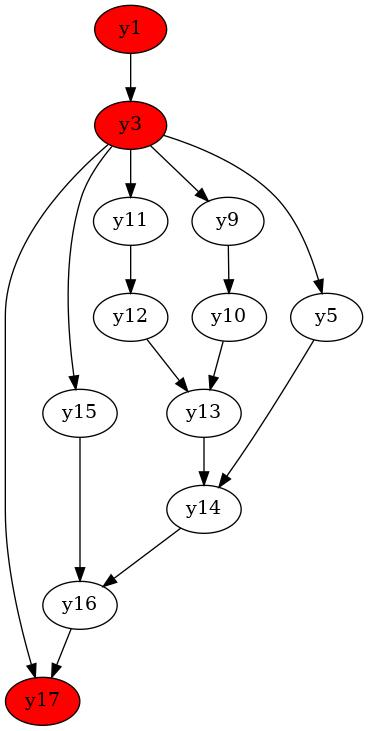
\includegraphics[width=0.25\textwidth]{graph_simple1.jpeg}
    \caption{Графовый вид простейшей системы}\label{graph_simple1}
\end{wrapfigure}

В предыдущей главе было описаны два принципиально отличающихся порядка вычисления: нормальный (в Coq тактика \texttt{lazy}) и аппликативный (в Coq тактика \texttt{cbv}) порядки, а также приведены их существенные недостатки. Рассмотрим, применимы ли эти недостатки к изучаемой задаче.

Основной недостаток аппликативного порядка --- неэффективная работа с "мёртвым кодом", блоками кода, результат редукции которых не влияет на итоговое вычисление. Могут ли такие блоки кода присутствовать во входных данных? Напомним, что входные данные состоят из набора уравнений $y_i = T_i$ и спецификации $P(y_0, y_n)$. Спецификация $P$ формально может быть любым предикатом, однако на практике в каждом конкретном доказательстве верификатора интересуют только некоторый срез системы, поведение отдельных частей программы. Из этого следует, что те части программы, которые не относятся к верифицируемому свойству, в терме $P(y_0, y_n)$ как раз и окажутся "мёртвым кодом". Вдобавок, при определённых стартовых состояниях $y_0$ некоторые ветки кода, отражённые в последующих уравнениях $y_i = T_i$, могут оказаться нерелевантными. К примеру, верификатора интересуют только стартовые состояние, при которых некоторое булевое поле равно \texttt{true}, тогда \texttt{else}-ветки соответствующих условных операторов окажутся мёртвым кодом. Таким образом, недостатки аппликативного порядка применимы к этой задаче в полной мере.

Основным недостатком же нормального порядка (особенно версии без мемоизации) является дублирование работы при преждевременной подстановке аргументов. Поскольку определение рассматриваемой системы уравнений разрешает в $T_i$ использовать любые $y_j$ для $j < i$, такое дублирование в теории может быть значительным. Чтобы изучить свойства реально рассматриваемых систем, был разработан графовый визуализатор. На рисунке \ref{graph_simple1} представлен графовый вид системы уравнений, построенной по простейшему линейному блоку кода (тест из множества Simple при n = 1, подробнее см. в разделе \ref{dataset}). Ребро $(y_i, y_j)$ означает, что в $T_j$ используется $y_i$, а красным выделены вершины, соответствующие глобальным состояниям системы.

\begin{wrapfigure}{l}{0.25\textwidth}
    \centering
    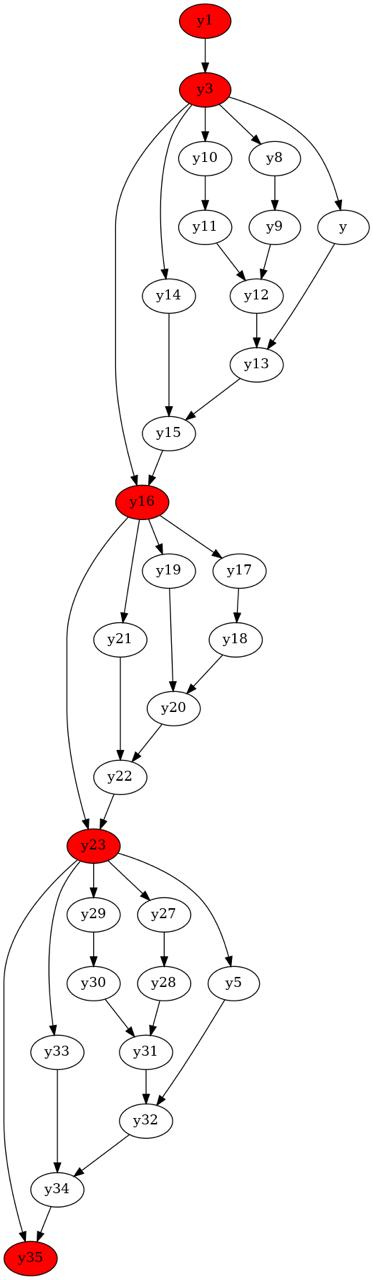
\includegraphics[width=0.25\textwidth]{graph_simple2.jpeg}
    \caption{Графовый вид системы из двух блоков кода}\label{graph_simple2}
\end{wrapfigure}

Если бы этот граф имел вид "бамбука", то есть если бы исходящая и входяшая степень каждой вершины была бы не больше одного, то можно было бы заключить, что нормальный порядок подходит отлично, так как подстановка не дублирует работу и мемоизация не требуется. Однако даже на простейшем линейном коде наблюдается достаточно ветвистый граф. А именно, существуют пять различных путей из $y_3$ в итоговое состояние $y_{17}$, то есть в худшем случае работа по редукции $y_3$ будет продублирована пять раз. Отметим, что $y_3$ соответствует глобальному состоянию системы, то есть является относительно большим термом, и дублирование его редукции даже несколько раз нежелательно.

На рисунке \ref{graph_simple2} представлен граф, построенный на основе двух блоков кода из предыдущего примера, с небольшой соединительной конструкцией между ними (тест из множества Simple при n = 2). Этот граф иллюстрирует, что число путей из стартовой вершины в итоговую, а значит, и потенциальное дублирование работы, становится экспоненциальным при увеличении размеров кода. Напомним, что код для этих иллюстраций взят упрощенный, на реальных примерах, особенно с разветвлением кода по условным операторам дублирование может быть ещё сильнее. Таким образом, при выборе нормального порядка необходима мемоизация, иначе замедление будет экспоненциальным, что недопустимо.

Итак, оба подхода имеют свои недостатки, и предварительный анализ входных данных показывает, что для рассматриваемой задачи оба недостатка --- "мёртвый код" и дублирование при подстановке --- применимы в полной мере. Дублирование при подстановке частично решается мемоизацией, однако эта техника создаёт определённые накладные расходы, и до перехода к экспериментам неочевидно, будет ли эти расходы стоить оптимизации по "мёртвому коду" по сравнению с аппликативным порядком. Соответственно, при дальнейшей разработке стратегий будут использоваться оба порядка и идеи, связанные с каждым из них.

\subsection{Базовые стратегии}

TODO

\subsection{Стратегии, основанные на декомпозиции}

TODO

\subsection{Дальнейшие оптимизации}

TODO

\subsection{Работа с условными операторами}

TODO

\subsection{Выводы и результаты по главе}

TODO

\end{document}
